\section{IR Based Conversation}
\subsection{IR Based Conversation}


\begin{frame}[shrink=10]{IR-Based Conversation}
\begin{multicols}{2}
\begin{itemize}
	\item IR based mostly used in the short-text conversation\footnote{Zongcheng Jia, Zhengdong Lub, Hang Li, An Information Retrieval Approach to Short Text Conversation, arXiv:1408.6988v1  [cs.IR]  29 Aug 2014}
	\item The corpus contains different pairs of post-comments or question answers
	\item[*] Given a question, and the set of documents, the task is to find the answer from the span of text from extracted paragraphs
\end{itemize}
For every given query $q$, there could be zero or more post-comment pairs $(p,r)$
The best response to the query $q$ is picked up based on the ranks of the retrieved pairs using
\begin{equation}
\hat{r} = \underset{(p,r)}{argmax}Score (q,(p,r))
\end{equation}
where $Score(.)$ is the sum of all score of the features
\begin{equation}
Score(q,(p,r)) = \sum_{i\in \Omega}^{}w_i\phi_i(q,r)
\end{equation}
where $\phi_i(.)$ and $w_i$ are the score and weight of the $i^{th}$ feature and $\Omega$ is the total number of features, respectively. Here the features could be TF*IDF of the word found in the \{q,(p,r)\}
\end{multicols}

\end{frame}

\begin{frame}{IR based Modeling - Architecture}


\begin{multicols}{2}
	\begin{center}
	\includegraphics[width=0.8\linewidth]{./Images/IR-basedCM}
\end{center}
\begin{itemize}
	\item 	\underline{Query-Response Similarity}:
	Here the similarity between the query and the candidate responses are computed using similarity measures such as cosine similarity
	\begin{equation}
	Similarity(q,r) = \dfrac{q^Tr}{||q||.||r||}
	\end{equation}
	\item 	\underline{Query-Post Similarity}:
	Here the similarity between the query and the candidate responses are computed using similarity measures such as cosine similarity
	\begin{equation}
	Similarity(q,p) = \dfrac{q^Tp}{||q||.||p||}
	\end{equation}

\end{itemize}
These similarity measures are proposed with the assumption that the there is some alignment of variables between query and posts and query and responses

\end{multicols}
\end{frame}

%\begin{frame}{TF*IDF Tables}
%\begin{table}
%	\tablename{TF*IDF for Posts}
%
%	\begin{tabular}{|c|c|c|c|c|}
%		\hline
%		&P1&p2&\ldots&Pn\\
%		Query Terms&&&&\\
%		\hline
%		$T_1$&&&&\\
%		$T_2$&&&&\\
%		$\ldots$&&&&\\
%		$T_m$&&&&\\
%		\hline
%	\end{tabular}
%\end{table}
%\begin{table}
%	\tablename{TF*IDF for Responses}
%
%	\begin{tabular}{|c|c|c|c|c|}
%		\hline
%		&P1&p2&\ldots&Pn\\
%		Query Terms&&&&\\
%		\hline
%		$T_1$&&&&\\
%		$T_2$&&&&\\
%		$\ldots$&&&&\\
%		$T_m$&&&&\\
%		\hline
%	\end{tabular}
%\end{table}
%\end{frame}
%

\begin{frame}{Learning To Rank}
\begin{figure}
	\centering
	\includegraphics[width=0.7\linewidth]{./Images/LearningToRank}
	\label{fig:learningtorank}
\end{figure}

\end{frame}
\begin{frame}{IR Based Conversations}
The main drawbacks of the retrieval-based method are the following
\begin{itemize}
	\item The Post,responses pairs are canned and it is hard to customize for the particular text or requirement from the task, e.g., style or attitude
	\item The use of matching features alone is usually not sufficient for distinguishing positive responses from negative ones, even after time consuming feature engineering.  (e.g., a penalty due to mismatched named entities is difficult to be incorporated into the model)
\end{itemize}

\end{frame}
